\documentclass[t]{beamer}
\usetheme{Copenhagen}
\setbeamertemplate{headline}{} % remove toc from headers
\beamertemplatenavigationsymbolsempty

\usepackage{amsmath, tikz, pgfplots, tcolorbox, xcolor, marvosym}
\pgfplotsset{compat = 1.16}

\tikzstyle{input} = [circle, text centered, radius = 1cm, draw = black]
\tikzstyle{function} = [rectangle, text centered, minimum width = 2cm, minimum height = 1cm, draw = black]

\title{Intro to Functions}
\author{}
\date{}

\AtBeginSection[]
{
  \begin{frame}
    \frametitle{Objectives}
    \tableofcontents[currentsection]
  \end{frame}
}

\begin{document}

\begin{frame} 
\maketitle
\end{frame}

\section{Determine if a relation is a function.}

\begin{frame}{Relations and Functions}
\begin{tcolorbox}[colback=red!15!white, colframe=red!60!black, title=Relations]
A \textbf{relation} is a set of ordered pairs.
\end{tcolorbox}
\vspace{1cm}	\pause

\begin{tcolorbox}[colback=red!15!white, colframe=red!60!black, title=Domain]
The \textbf{domain} is the set of all input values (usually $x$) of a relation.
\end{tcolorbox}
\end{frame}

\begin{frame}{Relations and Functions}
\begin{tcolorbox}[colback=red!15!white, colframe=red!60!black, title=Range]
The \textbf{range} is the set of all output values (usually $y$) of a relation.
\end{tcolorbox}
\vspace{1cm}	\pause
\begin{tcolorbox}[colback=red!15!white, colframe=red!60!black, title=Function]
A \textbf{function} is a relation is which each element of the domain has only 1 element in the range.
\end{tcolorbox}
\end{frame}

\begin{frame}{Example 1}
Determine whether each relation represents a function. For those that do, state the domain and range.	\newline\\
(a) \quad $\{(1,5), \, (2, 5), \, (3, 7), \, (4, 8)\}$	\newline\\	
\onslide<2->{All $x$-coordinates are different.\quad}
\onslide<3->{Is a function.}	\newline\\
\onslide<4->{Domain: 1, 2, 3, 4} \newline\\
\onslide<5->{Range: 5, 7, 8}
\end{frame}

\begin{frame}{Example 1}
(b) \quad $\{(5,1), \, (5,2), \, (7,3), \, (8,4)\}$	\newline\\
\onslide<2->{$x$-coordinates are not all different. \quad}
\onslide<3->{Is \textbf{not} a function.}
\end{frame}

\begin{frame}{Vertical Line Test}
It is also possible to determine if a relation is a function visually by using the \alert{vertical line test}:	\newline\\	\pause

\begin{tcolorbox}[colback=white!50!green, title=\textbf{Vertical Line Test}]
If every vertical line drawn hits the graph \underline{\textbf{at most once}}, then the relation is a function.
\end{tcolorbox}
\end{frame}

\begin{frame}{Example 1a Passes V.L.T.}
\begin{center}
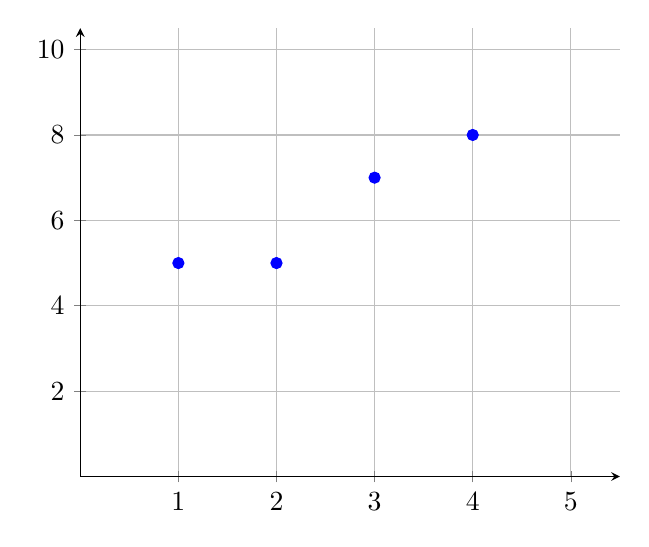
\begin{tikzpicture}
\begin{axis}[
	axis lines = middle,
	grid=both,
	xmin = 0, xmax = 5.5,
	ymin = 0, ymax = 10.5
]
\addplot[color=blue, mark = *, only marks] coordinates {(1,5) (2,5) (3,7) (4,8)};
\end{axis}
\end{tikzpicture}
\end{center}
\end{frame}

\begin{frame}{Example 1b Fails V.L.T.}
\begin{center}
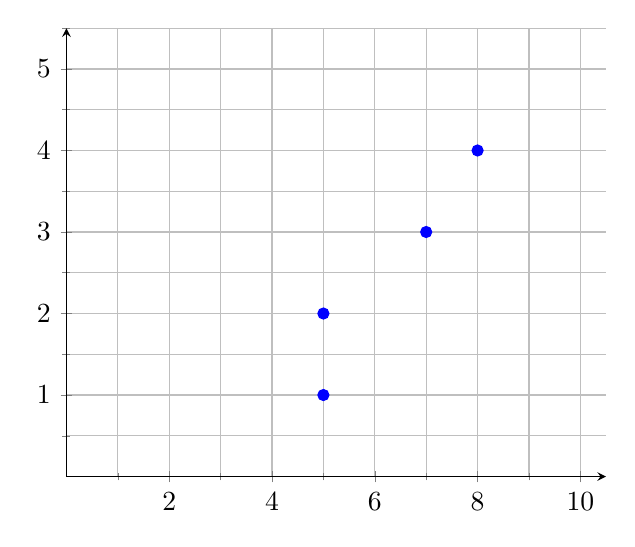
\begin{tikzpicture}
\begin{axis}[
	axis lines = middle,
	grid=both, minor tick num = 1,
	xmin = 0, xmax = 10.5,
	ymin = 0, ymax = 5.5
]
\addplot[color=blue, mark = *, only marks] coordinates {(5,1) (5,2) (7,3) (8,4)};
\end{axis}
\end{tikzpicture}
\end{center}
\end{frame}

\begin{frame}{Example 2}
Determine whether the graph of each represents a function.	\newline\\
(a) \newline\\
\begin{minipage}{0.5\textwidth}
\begin{tikzpicture}[domain = -1.5:1.5]
	\draw [<->] (-2,0) -- (2,0);
	\node at (2,0) [anchor = west] {\tiny $x$};
	\draw [<->] (0,-2) -- (0,2);
	\node at (0,2) [anchor = west] {\tiny $y$};
	\draw [<->, color = blue, very thick] plot(\x, {-1/2*\x-1/2});
\end{tikzpicture}
\end{minipage}
\begin{minipage}{0.4\textwidth}
\onslide<2->{Is a function}
\end{minipage}
\end{frame}

\begin{frame}{Example 2}
(b) \newline\\
\begin{minipage}{0.5\textwidth}
\begin{tikzpicture}[domain = -1.5:1.5]
	\draw [<->] (-2,0) -- (2,0);
	\node at (2,0) [anchor = west] {\tiny $x$};
	\draw [<->] (0,-2) -- (0,2);
	\node at (0,2) [anchor = west] {\tiny $y$};
	\draw [<->, color = blue, very thick] plot(\x, {-1/2*\x*\x+1/2});
\end{tikzpicture}
\end{minipage}
\begin{minipage}{0.4\textwidth}
\onslide<2->{Is a function}
\end{minipage}
\end{frame}

\begin{frame}{Example 2}
(c) \newline\\
\begin{minipage}{0.5\textwidth}
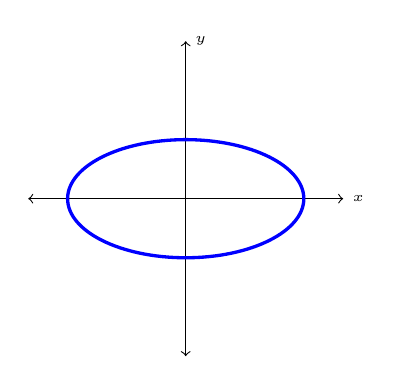
\begin{tikzpicture}
	\draw [<->] (-2,0) -- (2,0);
	\node at (2,0) [anchor = west] {\tiny $x$};
	\draw [<->] (0,-2) -- (0,2);
	\node at (0,2) [anchor = west] {\tiny $y$};
	\draw [color = blue, very thick] (0,0) ellipse (1.5 and 0.75);
\end{tikzpicture}
\end{minipage}
\begin{minipage}{0.4\textwidth}
\onslide<2->{Is not a function}
\end{minipage}
\end{frame}

\section{Evaluate a function using function notation.}

\begin{frame}{Functions}
Think of a function as a \alert{machine}. \newline\\	\pause
You give the function (machine) a value (input), it will process that value, and then return a value back to you (output). \newline\\	\pause

For instance, if you input 10 into the $x^2$ function, it will return $10^2$, or 100:	\newline\\
\begin{center}
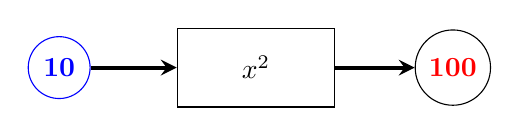
\begin{tikzpicture}[node distance = 2.5 cm]
\node (inputVal) [input, color=blue] {\color{blue}\textbf{10}};
\node (func) [function, right of = inputVal] {$x^2$};
\node (outputVal) [input, right of = func] {\color{red}\textbf{100}};

\draw [->, >=stealth, thick, line width = 1.5] (inputVal) -- (func);
\draw [->, >=stealth, thick, line width = 1.5] (func) -- (outputVal);
\end{tikzpicture}
\end{center}
\end{frame}

\begin{frame}{Function Notation}
A function can be described using \alert{function notation}. \newline\\ \pause
$f(x)$ represents the value of the function when the value of $x$ is substituted into it.	\newline\\	\pause
We can use other notations for functions including, but not limited to
\[ g(x) \quad h(x), \quad f(n) \quad f\left(\text{\Smiley}\right) \]
\pause \newline\\
When we substitute a value for the variable and evaluate it, that is called {\color{blue}\textbf{evaluating the function}}.
\end{frame}

\begin{frame}{Example 3}
Evaluate $f(2), \, f(-2), \, \text{and } f(0)$ for each.	\newline\\
(a) \quad $f(x) = 2x+3$	
\begin{align*}
\onslide<2->{f(2) &= 2(2) + 3} \\
\onslide<3->{&= 7} \\[10pt]
\onslide<4->{f(-2) &= 2(-2) + 3} \\
\onslide<5->{&= -1} \\[10pt]
\onslide<6->{f(0) &= 2(0) + 3} \\
\onslide<7->{&= 3}
\end{align*}
\end{frame}

\begin{frame}{Example 3}
Evaluate $f(2), \, f(-2), \, \text{and } f(0)$ for each.	\newline\\
(b) \quad $f(x) = 3x^2-1$	
\begin{align*}
\onslide<2->{f(2) &= 3(2)^2-1} \\
\onslide<3->{&= 11} \\[10pt]
\onslide<4->{f(-2) &= 3(-2)^2-1} \\
\onslide<5->{&= 11} \\[10pt]
\onslide<6->{f(0) &= 3(0)^2-1} \\
\onslide<7->{&= -1}
\end{align*}
\end{frame}

\begin{frame}{Example 3}
(c) \newline\\
\begin{minipage}{0.6\textwidth}
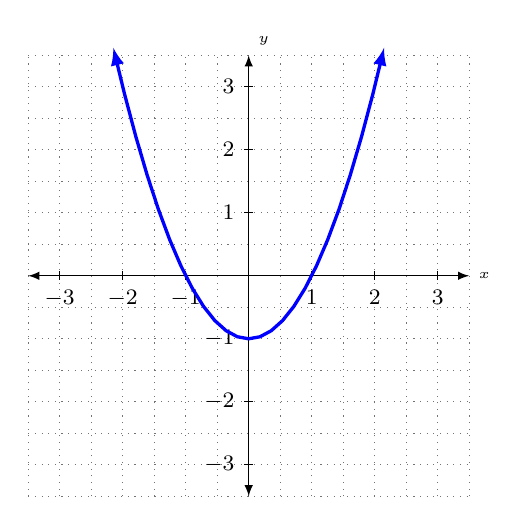
\begin{tikzpicture}[scale=0.8, domain = -2.15:2.15]
	\draw [step = 0.5cm, color = gray!110, dotted] (-3.5,-3.5) grid (3.5,3.5);
	\draw[<->, > = latex] (-3.5,0) -- (3.5,0);
	\node at (3.5,0) [anchor = west] {\tiny $x$};
	\draw[<->, > = latex] (0,-3.5) -- (0,3.5);
	\node at (0,3.5) [anchor = south west] {\tiny $y$};
	\foreach \x in {-3,-2,-1,1,2,3}
	\draw[shift = {(\x,0)}] (0pt,2pt) -- (0pt, -2pt) node[below] {\footnotesize $\x$};
	\foreach \y in {-3,-2, -1, 1, 2, 3}
	\draw[shift = {(0,\y)}] (2pt,0pt) -- (-2pt,0pt) node[left] {\footnotesize $\y$};
	\draw [<->, > = latex, color = blue, very thick]	plot (\x, {\x*\x - 1});
\end{tikzpicture}
\end{minipage}
\begin{minipage}{0.25\textwidth}
\begin{align*}
\onslide<2->{f(2) &= 3} \\[12pt]
\onslide<3->{f(-2) &= 3} \\[12pt]
\onslide<4->{f(0) &= -1}
\end{align*}
\end{minipage}
\end{frame}

\end{document}